\documentclass{article}

\usepackage[
backend=biber,
style=numeric,
sorting=ynt
]{biblatex}
\addbibresource{refs.bib}

\usepackage{soul}
\usepackage{ifthen}
\usepackage[makeroom]{cancel}
\usepackage{amsthm}
\usepackage{amsmath}
\usepackage{amssymb}
\usepackage{mathtools}
\usepackage{needspace}
\usepackage{etoolbox}
\usepackage{listofitems}
\usepackage{xstring}
\usepackage{graphicx} % Required for inserting images
\usepackage{tikz}
\usetikzlibrary{patterns}
\usetikzlibrary{external}

\newtheorem{theorem}{Theorem}
\newtheorem{definition}{Definition}
\newtheorem{lemma}{Lemma}
\newtheorem{example}{Example}

\preto{\lemma}{\needspace{4cm}}
\preto{\section}{\needspace{5cm}}
\preto{\subsection}{\needspace{3cm}}
\preto{\example}{\needspace{3cm}}

\title{Heart of the Four Color Theorem}
\author{Timothy van der Valk}
\date{November 2024 - January 2025}

\newcommand{\I}{\text{I}}
\newcommand{\II}{\text{II}}
\newcommand{\compat}{\implies}
\newcommand{\ncompat}[1]{\stackrel{#1}{\compat}}
\newcommand{\digitToNum}[1]{\the\numexpr#1\relax}
\newcommand{\scheme}[2]{
    \readlist*\mylist{#2}
     \tikz[baseline]{ 
        \foreach \x [count=\i] in {#1} {
            \coordinate (\i) at (0.3*\i, 0.225); \node[text height=0mm] at (0.3*\i,0) {$\x$};
        } 
        \foreachitem \z \in \mylist {
            \StrChar{\z}{1}[\left]
            \StrChar{\z}{2}[\right]
            \StrChar{\z}{3}[\color]
            \StrChar{\z}{4}[\cross]
            \path (\left) edge[bend left=45] node[above, yshift=-2]{\small 
            \ifthenelse{\equal{\cross}{-}}{$\cancel{\color}$}{$\color$}
            } (\right);
        }
    }
} 

\begin{document}

\maketitle

A new proof of the four-color theorem has been given by Thomas et al \cite{thomas} in 1995 as a response to the Appel and Haken proof from 1976. Both proofs of the four-color theorem depend on three smaller theorems and a set of configurations that together contradict the existence of a minimal counterexample. The difference is that the new proof has a set of 633 configurations compared to 1476 members of the old one.

This document elaborates on the key concepts and results of reducibility underlying the four color theorem. The theory is built up from an intuitive and chronological point of view. Every definition is strongly motivated before being introduced. Ring reducibility results of Birkhoff have been rewritten using solid definitions and new notation and figures are included for most intuitive explanations. In addition, several examples of the types of reducibility are given. The C-reducibility of the Birkhoff diamond is proven and its full reducibility structure is visualised.

\tableofcontents

\pagebreak
\section{Introduction}

The four-color theorem is proven by disproving the existence of minimal counterexamples. Let us begin by defining such a minimal counterexample.
\begin{definition}
A graph $G$ is a minimal counterexample to the four-color theorem if $G$ is not four-colorable but any graph $H$ of lower weight $|V(H)|+|E(H)|$ is.
\end{definition}

All minimal counterexamples we mention will be those of the four-color theorem.
The three theorems to the four-color theorem are then as follows. We leave further definitions to Sections \ref{sec:birkhoff} and \ref{sec:dreduce}.

\begin{theorem}
Minimal counterexamples are Birkhoff graphs.
\end{theorem}

\begin{theorem}
Minimal counterexamples do not contain configurations.
\end{theorem}

\begin{theorem}
Birkhoff graphs contain a configuration.
\end{theorem}

Clearly these three results contradict each other. Minimal counterexamples are proven to have no configurations, but subsequently through Birkhoff graphs, do in fact have configurations. As a consequence, there can not exist any minimal counterexamples and the four-color theorem is true. 

Theorem 1 is proven by hand in Section \ref{sec:birkhoff}. Theorem 2 and 3 require a computer to verify all cases. Birkhoff graphs are also called "internally 6-connected triangulations" in literature, but we will use the former for readability.

\section{Ring Reducibility}
\label{sec:birkhoff}

Before 1913, the only known reductions of maps we're the reductions to triangulations and the reduction of multiply-connected regions to fewer regions (holed regions). In 1913, Birkhoff \cite{birkhoff} proved a new reduction result for \textit{rings} that seperate two parts of a map. This result spurred new developments in the reduction of graphs that opened the path towards reducible configurations and finally the proof of Appel and Haken in 1976.

\subsection{Rings and chains}

We will use the term \textit{map} to refer to a map of connected \textit{regions} that we wish to four-color. From such a map we can construct a \textit{planar graph} where each region represents a vertex. We will be working with planar graphs in all our proofs, but might sometimes mention maps for intuition.

Let $|G|$ be the number of vertices of $G$. Then we have the following well-known reduction to triangulations.

\begin{theorem}
\label{thm:triang}
    Given a planar graph $G$ with a non-triangular bounded face. Then the coloring of $G$ can be reduced to a graph on $H$ less vertices.
\end{theorem}
\begin{proof}
    A non-triangular bounded face of $G$ corresponds to a cycle of size greater than three in $G$. Combine any two non-neighboring vertices in this cycle to form a graph on one less vertex $H$. Given a coloring of $H$, we may color the two contracted vertices the same to obtain a coloring of $G$.
\end{proof}

Let us now define rings.

\begin{definition}
    A ring of $n$ vertices $R_n$ in a planar graph $G$ is an induced cycle of $G$ that encloses at least one vertex.
\end{definition}

The key property of rings is that they seperate the full graph $G$ in three parts $M_1$, $R$ and $M_2$. That is, $G$ is of the form $G = M_1 + R + M_2$ where the order of addition indicates how each part is connected to the other.

\begin{figure}[!ht]
    \centering
        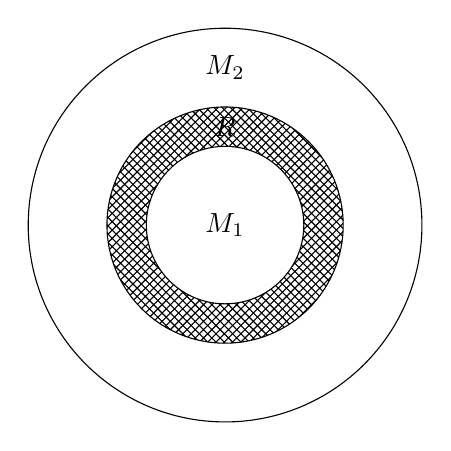
\begin{tikzpicture}
        \draw[fill=white] (0,0) circle (2.5cm);
        \draw[fill opacity=0.4, pattern=crosshatch] (0,0) circle (1.5cm);
        \draw[fill=white] (0,0) circle (1cm);
        \node at (0, 1.25) {$R$};
        \node at (0, 2) {$M_2$};
        \node at (0, 0) {$M_1$};
    \end{tikzpicture}
    \caption{The graph $M_1 + R + M_2$.}
\end{figure}

To reduce a ring like this, we ideally want to color $M_1+R$ and $M_2+R$ in such a way that the colors on $R$ are the same. Then we can glue the two colorings together to form a coloring of $G$.

It might however, not always be possible to reduce a graph with a ring $R$ to $M_1+R$ and $M_2+R$. For a weaker result, we may try reducing to slightly larger graphs, $M_1+R+A_1$ and $M_2+R+A_2$ where $A_1$ and $A_2$ are two arbitrary graphs of at most $k$ vertices that are connected to $R_n$.

This is a weaker result, because if we allow $k$ to be big enough, we can simply set $A_1 = M_2$ and $A_2 = M_1$ to reduce to twice $M_1 + R + M_2$, which obviously has a common coloring on the ring. Let us define this generalization of ring reducibility.

\begin{definition}
    A ring $R_n$ is said to be k-reducible if for all planar graphs $G$ containing the ring $R_n$, the coloring of $G$ can be reduced to the coloring of $M_1+R_n+A_1$ and $M_1+R_n+A_2$ with $A_1$ and $A_2$ two arbitrary planar graphs on at most $k$ vertices that are connected to $R_n$.
\end{definition}

For example, the following is a trivial result.

\begin{example}
    The rings $R_1, R_2$ and $R_3$ are 0-reducible.
\end{example}

\begin{proof}
    The colorings only possible colorings on these rings (up to permutation) are $\{ a \}, \{ ab \}$ and $\{ abc \}$. Given a coloring of $M_1+R$ and $M_2+R$, we can simply permute the colors in both graphs to make the colorings agree on the ring. Hence we have 0-reducibility.
\end{proof}

Starting from the ring $R_4$, we briefly introduce two concepts to make the proof easier to follow. The first are Kempe-chains first introduced by Alfred Kempe.
\begin{definition}
    Given two colors $a,b$ and a coloring of a planar graph $G$. The $ab$-chain of a vertex $v$ in $G$ is the induced subgraph of $v$ and all vertices colored $a,b$ that are connected to $v$ directly or through other vertices colored $a,b$.
\end{definition}

In addition, we introduce a notation for writing down the colors on a ring $R$ and any chains that connect two vertices of the ring. We call these \emph{ring schemes}.

\begin{figure}[!ht]
    \centering
    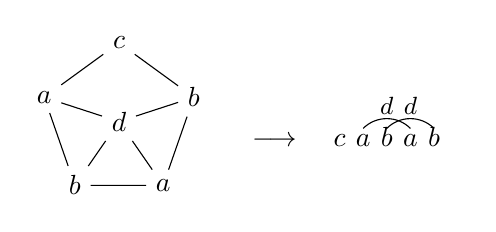
\begin{tikzpicture}
        \node (v1) at (0, 1) { $c$ };
        \node (v2) at (-0.95, 0.309) { $a$ };
        \node (v3) at (-0.56, -0.81) { $b$ };
        \node (v4) at (0.56, -0.81) { $a$ };
        \node (v5) at (0.95, 0.309) { $b$ };
        \node (x) at (0, 0) { $d$ };

        \draw (v1) -- (v2) -- (v3) -- (v4) -- (v5) -- (v1);
        \draw (v3) -- (x) -- (v5);
        \draw (v4) -- (x) -- (v2);

        \node (scheme) at (3, 0) { $\longrightarrow$ \scheme {c,a,b,a,b}{24d, 35d} };
    \end{tikzpicture}
    \\
    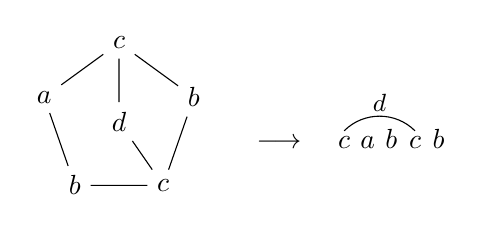
\begin{tikzpicture}
        \node (v1) at (0, 1) { $c$ };
        \node (v2) at (-0.95, 0.309) { $a$ };
        \node (v3) at (-0.56, -0.81) { $b$ };
        \node (v4) at (0.56, -0.81) { $c$ };
        \node (v5) at (0.95, 0.309) { $b$ };
        \node (x) at (0, 0) { $d$ };

        \draw (v1) -- (v2) -- (v3) -- (v4) -- (v5) -- (v1);
        \draw (v1) -- (x) -- (v4);

        \node (scheme) at (3, 0) { $\longrightarrow$ \scheme {c,a,b,c,b}{ 14d }};
    \end{tikzpicture}
    \\
    \begin{tikzpicture}
        \node (v1) at (0, 1) { $a$ };
        \node (v2) at (1, 0) { $b$ };
        \node (v3) at (0, -1) { $c$ };
        \node (v4) at (-1, 0) { $b$ };
        \node (x1) at (-0.35, 0) { $c$ };
        \node (x2) at (0.35, 0) { $a$ };

        \draw (v1) -- (x1) -- (x2) -- (v3);
        \draw (v1) -- (v2) -- (v3) -- (v4) -- (v1);
        \node (scheme) at (3, 0) { $\longrightarrow$ \scheme {a,b,c,b}{ 13 }};
    \end{tikzpicture}
    \caption{Examples of rings $R_4$ and $R_5$ with chains. A layout of chains on the ring can be indicated with the ring scheme notation. }
\end{figure}

The key property of ring schemes is that we may freely flip $ab$-chains for vertices that are seperated by a $cd$-chain, since these $ab$-chains can never be connected.

\begin{definition}
    A ring scheme $x$ implies another ring scheme $y$ if $y$ can be obtained from $x$ by flipping an $ab$-chain. In this case we write $x \compat y$.
\end{definition}

For example, in the earlier figure of a ring scheme on $R_4$ we have

\begin{equation*}
    \scheme{a,b,c,b}{{13}} \compat \scheme{a,b,c,d}{{13}}.
\end{equation*}

We will now use the concepts of chains and ring schemes to prove that the ring $R_4$ is 0-reducible and the ring $R_5$ 1-reducible.

\subsection{The ring $R_4$ is 0-reducible}

In this section we will prove the following theorem:

\begin{theorem}
    The ring $R_4$ is 0-reducible.
\end{theorem}
\begin{proof}

Let us consider the possible ring colorings I and II of the graphs $M_1+R_4$ and $M_2+R_4$. Since the ring in this case is a 4-cycle, we may color two of its vertices the same by Theorem \ref{thm:triang}. We can merge either $v_1$ and $v_3$ or $v_2$ and $v_4$ to obtain the colorings $a{*}a{*}$ and ${*}a{*}a$, where the ${*}$-vary per coloring.

If any of these two colorings in I and II are equal (up to permutation), we are done. Otherwise, we may assume that

\begin{equation}
    \{ abab \}\subset \I \quad \text{and}  \quad \{ abac, baca \} \subset \II.
\end{equation}

Now suppose that there is an $ad$-chain between $v_1$ and $v_3$ in $I(abab)$. We are allowed to flip the $bc$-chain of $v_4$ without affecting $v_2$ because the $ad$-chain in complementary colors seperates them. Thus we obtain

\begin{equation}
    \I(abab) = \scheme{a,b,a,b}{13d} \compat \II(abac)
\end{equation}

If there is no such $ad$-chain between $v_1$ and $v_3$, then likewise we are allowed to flip the $ad$-chain of $v_3$ without affecting $v_1$ to obtain

\begin{equation}
    \I(abab) = \scheme{a,b,a,b}{13d-} \compat \I(abcb) = \II(baca).
\end{equation}

In any case, we obtain a common coloring between I and II. Therefore the ring $R_4$ is 0-reducible.
\end{proof}

\subsection{The ring $R_5$ is 1-reducible}

A know result is that every planar graph has a vertex $v$ of degree at most 5. If we apply the reduction to triangulations, this means that the five vertices surrounding $v$ form the ring $R_5$. If $R_5$ we're 0-reducible, then every planar graph would be reducible and as a consequence, no minimal counterexamples could exist to the four color theorem.

This is an intuition as to why it might be hard to prove that $R_5$ is 0-reducible (we have tried). Instead we will prove the weaker 1-reducibility, this will turn out to be sufficient for subsequent work on the four color theorem.

\begin{theorem}
    The ring $R_5$ is 1-reducible.
\end{theorem}

\begin{proof}Let us consider the possible ring colorings I and II of $M_1 + R_5 + A_1$ and $M_2 + R_5 + A_2$. We must now take into account the graphs $A_1$ and $A_2$ on at most one vertex. The colorings depend on the amount of vertices in $A$

\emph{$A$ has one vertex}. In this case we have the sole vertex of $A$ connected to all vertices of the ring by definition. Because we assume four-colorability, the ring can only contain three colors and hence must be colored one of $\underline{c}abab$ where the vertex colored $\underline{c}$ is free to be any of the five vertices.

\emph{$A$ is empty}. In this case we have no vertices on the other side of the ring $R_5$. Because it is a 5-cycle, we may apply Theorem \ref{thm:triang} to merge any two opposing vertices thus coloring them the same. This results in five different colorings of the form $a{*}{*}a{*}$ where any two non-adjacent vertices may be colored $a$.

Therefore we assume the following colorings for I and II:

\begin{equation}
    \left\{ \begin{matrix}
        \text{one of}\;\underline{c}abab \; \text{with $c$ free}, \\
        \text{all of}\;a{*}{*}a{*} \; \text{with $a$  non-adjacent}
    \end{matrix}\right\} \subset \text{I, II}.
\end{equation}

Now we will prove that for these two sets, we can always deduce a common coloring on the ring $R_5$. To this end, we will prove two lemma's.

Let a vertex colored uniquely in one of $\underline{c}abab$ be called the \emph{marked vertex}, indicated by an underlined color. Let two colorings be called \emph{adjacent} if their marked vertices are adjacent.

\begin{lemma}
    \label{lem:r5_first}
    If I and II have a non-adjacent coloring, then they either have an adjacent coloring or a common coloring.
\end{lemma}

\begin{lemma}
    \label{lem:r5_second}
    If I and II have an adjacent coloring, then they have a common coloring.
\end{lemma}

\emph{Proof of Lemma \ref{lem:r5_first}}.
Let two non-adjacent colorings $\I(\underline{c}abab)$ and $\II(ab\underline{c}ab)$ be given. Suppose that a $bc$-chain connects $v_3$ and $v_5$ in $\II(ab\underline{c}ab)$. Then we obtain

\begin{equation}
    \label{eq:abcab}
    \II(ab\underline{c}ab) =\scheme{a,b,c,a,b}{35b} \compat \II(abcdb).
\end{equation}

If no such chain exists, then we may flip the $bc$-chain of $v_3$ to obtain

\begin{equation}
    \II(ab\underline{c}ab) = \scheme{a,b,c,a,b}{35b-} \compat \II(a\underline{c}bab) \;\; \text{adjacent to} \;\; \I(\underline{c}abab).
\end{equation}

Now to deal with the former coloring, we consider the coloring $\I({*}b{*}{*}b)$. The three unique possibilities for the colors lead to

\begin{equation}
    \begin{matrix*}[l]
        \I(abcdb) \quad\quad =&\II(abcdb) \; \text{from (\ref{eq:abcab}),}  \\
        \I(cbc\underline{d}b) \;\; \text{adjacent to}&\II(ab\underline{c}ab), \;  \\
        \I(db\underline{c}db) \quad\quad =&\II(ab\underline{c}ab).
    \end{matrix*}
\end{equation}

A similar argument holds for any other pair of non-adjacent colorings for I and II. Therefore we obtain either a common coloring or an adjacent coloring. These adjacent colorings are then treated by the second lemma $\qedsymbol$.

\vspace{1em}
\emph{Proof of Lemma \ref{lem:r5_second}}

Let two adjacent colorings $\I(\underline{c}abab)$ and $\II(a\underline{c}bab)$ be given. Suppose a $bd$-chain connects $v_3$ and $v_5$ in $\II(a\underline{c}bab)$. Then we obtain

\begin{equation}
    \II(a\underline{c}bab) = \scheme{a,c,b,a,b}{35d} \compat \I(\underline{c}abab).
\end{equation}

If no such chain exists, then we may flip the $bd$-chain of $v_3$ to obtain

\begin{equation}
    \label{eq:acdab}
    \II(a\underline{c}bab) = \scheme{a,c,b,a,b}{35d-} \compat \II(acdab).
\end{equation}

Now we consider the coloring $\I(a{*}{*}a{*})$. The three unique possibilities for the colors lead to

\begin{equation*}
    \begin{matrix*}[l]
        \I(acdab) \quad =& \II(acdab), \;\text{from (\ref{eq:acdab})},\\
        \I(ac\underline{d}ac) \; &\text{shifted two to right of $\I(\underline{c}abab)$}, \\
        \I(a\underline{c}dad) \quad =& \II(a\underline{c}bab).
    \end{matrix*}
\end{equation*}

By following this procedure, we end up with either a common coloring, or a coloring that is shifted two to the right.

We can repeat this procedure again with $\II(a\underline{c}bab)$ and $\I(ac\underline{d}ac)$, to obtain $\II(aba\underline{c}b)$. Another repetition yields another shifted coloring for I. Hence we obtain the pattern

\begin{equation}
    \I(\underline{c}abab) \rightarrow \I(ab\underline{c}ab) \rightarrow \I(abab\underline{c}) \rightarrow \I(a\underline{c}bab) = \II(a\underline{c}bab).
\end{equation}

A similar argument holds for any pair of adjacent colorings of I and II. Therefore, in all cases, we obtain a common coloring $\qedsymbol$.

\vspace{1em}
If the marked vertices are the same, we can simply permute colors to obtain a common coloring of I and II. Together with these two lemma's we will have covered all cases of marked vertices. Therefore the ring $R_5$ is 1-reducible.

\end{proof}

\subsection{Birkhoff graphs}

Now that we have proven two new reducibiliy results, we want to put them in the context of the four color theorem. In particular, we are interested in the nature of minimal counterexamples. Minimal counterexamples can not be reducible, because if they we're, we could reduce their coloring to a smaller graph that \emph{is} four colorable by minimality. Let $G$ be a minimal counterexample to the four-color theorem.

\emph{By 0-reducibility of $R_4$}, this means no vertex $v$ of $G$ can have four neighbours, since otherwise by triangulation, the neighbours of $v$ would form $R_4$ which is reducible.

\emph{By 1-reducibility of $R_5$}. In this case we can only reduce to a smaller graph if both sides of $R_5$, $M_1$ and $M_2$, have at least two vertices. Suppose the ring $R_5$ has a graph $M_1$ on one side, and a single vertex $v$ on the other. Then it is possible that one of our reduced graphs is $M_1 + R_5 + A_1$ with $|A_1|=1$, but this graph has exactly the same size as $G$. Therefore we did not achieve a size reduction. 

This means that we can only say with certainty that $G$ has no ring $R_5$ with more than two vertices on either side.
\\
A key definition in the three theorems for the four-color theorem is that of \emph{Birkhoff graphs}. These graphs are exactly the irreducible graphs $G$ we specified above.

\begin{definition}
    A Birkhoff graph $G$ is a planar triangulation without the ring $R_4$ and the ring $R_5$ of more than two vertices on either side.
\end{definition}

An equivalent definition is that of \emph{internally 6-connected triangulations}.

\begin{definition}
    An internally 6-connected triangulation is a graph $G$ where for any cutting set $X$ with $G\setminus X$ disconnected, $|X| \geq 6$ or $|X|=5$ with $G\setminus X$ having two components of which one is a single vertex.
\end{definition}

These two are equivalent because cuttings sets are the same as rings.
\\
Let us finish this section with one last result to test our intuition.

\begin{theorem}
    The four color theorem is equivalent to $R_5$ being 0-reducible.
\end{theorem}

\begin{proof}
\hfill\newline
$\Longrightarrow$ Suppose the four color theorem is true, then we know that any planar graph $M_1 + R_5 + M_2$ is four-colorable. Given such a four-coloring, we will obtain a common coloring for $M_1+R_5$ and $M_2+R_5$.\\
$\Longleftarrow$ Suppose that $R_5$ is 0-reducible. Given a minimal counterexample to the four color theorem $G$, then we have that there exists a vertex $v$ of degree at most five in $G$. Because $G$ is a triangulation, the neighbors of $v$ must form $R_5$. Because all rings smaller or equal to $R_5$ are 0-reducible, we may always reduce $G$ to two components $M_1+R_5$ and $v+R_5$, both of which are smaller than $G$. Therefore $G$ is four colorable and no minimal counterexample can exist.
\end{proof}

Since we already know that the four color theorem is true, we know that the ring $R_5$ is also 0-reducible. Because it might seem so easy to prove that $R_5$ is 0-reducible, it was in fact Alfred Kempe himself who gave the first false proof of the four color theorem. See \cite{kempe}.

Despite his failed proof, he continued on to introduce the concept of rings to mathematics on which this section is based, and these rings ended up at the heart of the four color theorem.
\section{D-Reducibility}
\label{sec:dreduce}

\subsection{Definitions}

The proof of the four-color theorem consists of proving that every graph has a certain subgraph that can be reduced to a smaller graph. So far, we have proven reducibility only for graphs containing the rings $R_4$ and $R_5$. The graphs that we we're left with we called Birkhoff graphs.

Since Birkhoff graphs already contain a lot of structure and information, our hopes are that every such Birkhoff graph contains \textbf{at least one subgraph of a finite set of reducible subgraphs}. We will call these subgraphs \textit{configurations}.

\begin{definition}
    A configuration is a triangulation where the outer vertices form a ring $R_n$ of size $n \geq 4$.
\end{definition}

An example of a configuration is the \textit{Birkhoff diamond} visible in Figure \ref{fig:diamond} of Section \ref{sec:diamond} which was proven to be reducible by Birkhoff \cite{birkhoff}.

We have seen the notion of one ring scheme \textit{implying} another by means of a flipping of color chains. Consider now a single coloring say $abab$ of $R_4$. By conditioning on the presence of an $ad$-chain, we obtain two implied colorings.

\begin{equation*}
    \scheme{a,b,a,b}{{13d}} \compat abac
    \quad\text{or}\quad
    \scheme{a,b,a,b}{13d-} \compat abcb.
\end{equation*}

We therefore know with certainty that $abab$ implies either $abac$ or $abcb$. In such a case we write $abab \compat \{ abac, abcb \}$.

\begin{definition}
    A ring coloring $x$ implies a set of ring colorings $\II$ if for some pair of colors $ab$, all possible $ab$-chain schemes on $x$ imply a coloring of $\II$. We write $x \compat \II$.
\end{definition}

We can extend this to a set of colorings $\I$ implying $\II$ if all colorings of $x \in \I$ imply $\II$.

\begin{definition}
    A set of ring colorings $\I$ implies another set of ring colorings $\II$ if every $x \in \I$ implies $\II$. We write $\I \compat \II$.
\end{definition}

If you think about these definitions for a while, you will realize that the proofs of ring reducibility in Section \ref{sec:birkhoff} are mostly about proving that one set of ring colorings implies another.

How can we utilize this concept of implied sets to define a notion of reducibility for configurations? Given a configuration $C$, let us start by defining the sets of possible ring colorings of $C$ and a ring $R_n$.

\begin{definition}
    Let $\Phi_0(C)$ be the set of all ring colorings of a configuration $C$. Let $\Phi(n)$ be the set of all ring colorings of $R_n$.
\end{definition}

Consider an arbitrary ring coloring $x \in \Phi(n)$. If $x \in \Phi_0(C)$, then clearly we may reduce this configuration. Now using the concept of implying sets, let $\Phi_1(C)$ be the largest set such that $\Phi_1(C) \implies \Phi_0(C)$. Then every coloring in $\Phi_1(C)$ can be turned into a coloring of $\Phi_0(C)$ regardless of the chains present. Thus if $x \in \Phi_1(C)$, we are again reducible.

We can continue constructing sets of higher-level implication $\Phi_n(C)$ and each of the colorings in these sets can be used to reduce our configuration. Note that these sets are increasing in size, containing the previous set as well. That is $\Phi_n(C) \subset \Phi_{n+1}(C)$. Since these sets can not grow bigger than the set of all ring colorings $\Phi(n)$, there exists a largest such set $\overline{\Phi}(C) = \Phi_k(C)$ for some $k > 0$.

Finally, our configuration is D-reducible if this maximal set $\overline{\Phi}(C)$ is the set of all possible ring colorings $\Phi(n)$. Since in this case every coloring can be converted into a coloring for $C$ with chain flips.  Let us now define this intuition properly. Starting with higher-order implication.

\begin{definition}
    A set of ring colorings I $n$-implies another set II written as $\I \ncompat{n} \II$ if for some sets $B_{i}$ with $0 < i < n$,

    \begin{equation*}
        I \compat B_{n-1} \compat  \ldots \compat B_{1} \compat \II.
    \end{equation*}
\end{definition}

Using this definition, we will define the $n$-implying sets of a configuration $C$.

\begin{definition}
    The $n$-implying set $\Phi_n(C)$ of a configuration $C$ is the largest set of ring colorings such that $\Phi_n(C) \ncompat{n} \Phi_0(C)$.
\end{definition}

Finally, we define the largest implying set simply as \textit{the} implying set.

\begin{definition}
    The implying set $\overline{\Phi}(C)$ of a configuration $C$ is the largest $n$-implying set $\Phi_n(C)$ for some $n$ of $C$.
\end{definition}

With all these definitions in place, we can define the notion of D-reducibility.

\begin{definition}
    A configuration $C$ of ring size $n$ is D-reducible if $\overline{\Phi}(C) = \Phi(n)$.
\end{definition}

\begin{figure}[!h]
    \centering
    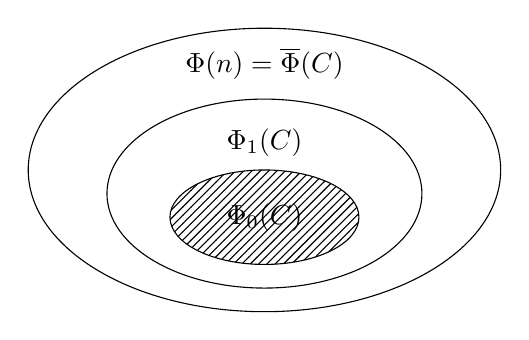
\begin{tikzpicture}[scale=1.0]
        \draw (0, 0) ellipse (3cm and 1.8cm);
        \draw (0, -0.3) ellipse (2cm and 1.2cm);
        \draw[fill opacity=0.4, pattern=north east lines] (0, -0.6) ellipse (1.2cm and 0.6cm);

        \node at (0.0, -0.6) { $\Phi_0(C)$ };
        \node at (0.0, 0.35) { $\Phi_1(C)$ };
        \node at (0, 1.35) { $\Phi(n) = \overline{\Phi}(C)$ };
    \end{tikzpicture}

    \caption{D-reducibility requires that all ring colorings can be converted to a valid ring coloring of $C$ in $\Phi_0(C)$.}
\end{figure}

Let us now view some simple examples of D-reducibility. A detailed example about the Birkhoff diamond can be found in Section \ref{sec:diamond}.

\subsection{Reducibility of the 4-star and 5-star}

For examples with and without D-reducibility, we look at the 4-star and 5-star respectively. They are pictured below.

\begin{figure}[!h]
    \centering
    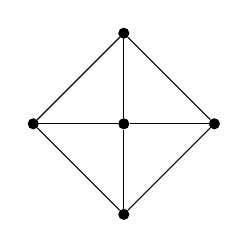
\begin{tikzpicture}[scale=1.15]
        \node[circle, fill, scale=0.015cm] (c) at (0, 0) {};
        \node[circle, fill, scale=0.015cm] (l1) at (1, 0) { };
        \node[circle, fill, scale=0.015cm] (l2) at (0, -1) { };
        \node[circle, fill, scale=0.015cm] (l3) at (-1, 0) {};
        \node[circle, fill, scale=0.015cm] (l4) at (0, 1) {};

        \draw (c) -- (l1);
        \draw (c) -- (l2);
        \draw (c) -- (l3);
        \draw (c) -- (l4);
        \draw (l1) -- (l2) -- (l3) -- (l4) -- (l1);

    \end{tikzpicture}
    \hspace{0.5cm}
    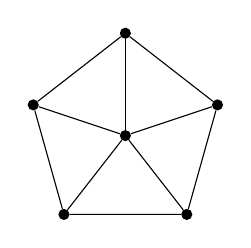
\begin{tikzpicture}[scale=1.3]
        \node[circle, fill, scale=0.015cm] (c) at (0, 0) {};
        \node[circle, fill, scale=0.015cm] (l1) at (0, 1) { };
        \node[circle, fill, scale=0.015cm] (l2) at (0.9, 0.30) { };
        \node[circle, fill, scale=0.015cm] (l3) at (0.6, -0.77) {};
        \node[circle, fill, scale=0.015cm] (l4) at (-0.6, -0.77) {};
        \node[circle, fill, scale=0.015cm] (l5) at (-0.9, 0.30) {};

        \draw (c) -- (l1);
        \draw (c) -- (l2);
        \draw (c) -- (l3);
        \draw (c) -- (l4);
        \draw (c) -- (l5);
        \draw (l1) -- (l2) -- (l3) -- (l4) -- (l5) -- (l1);
    \end{tikzpicture}
    \caption{The 4-star and the 5-star.}
\end{figure}

For the 4-star, we know that the only colorings it allows on the ring are those with three colors or less. Hence

\begin{equation}
    \Phi_0(\text{4-star}) = \{ abab, abac, baca \}.
\end{equation}

However, the set of all ring colorings of $R_4$ also includes the coloring $abcd$.

\begin{equation}
    \Phi(4) = \{ abab, abac, baca, abcd \}.
\end{equation}

Therefore, to prove D-reducibility, we must show that $abcd \in \Phi_n(\text{4-star})$ for some $n$-implying set. In this case we obtain that

\begin{equation}
    \scheme{a,b,c,d}{13a} \compat abcb \quad \text{or} \quad \scheme{a,b,c,d}{13a-} \compat abad.
\end{equation}

Both of these colorings are in $\Phi_0(\text{4-star})$ up to permutation. Therefore

\begin{equation*}
    \Phi_1(\text{4-star}) = \{ abcd \}.
\end{equation*}

Hence $\overline{\Phi}(\text{4-star}) = \Phi(4)$ and we can conclude that the 4-star is D-reducible.

However, the 5-star is unfortunately not D-reducible (this would also prove the four color theorem). The problem can quickly be seen from the fact that any chain on a 4-coloring like $abcad$ implies both a 3-coloring and 4-coloring.

\begin{equation*}
    \scheme{a,b,c,a,d}{35c} \compat abcbd \quad \text{or} \quad \scheme{a,b,c,a,d}{35c-} \compat abcbd.
\end{equation*}

The actual proof involves evaluating many cases, which can be done with a computer.

Next we treat C-reducibility that serves as the final form of reducibility required for the four-color theorem.
\section{C-Reducibility}
\label{sec:creduce}

The original proof of the four color theorem used an unavoidable set of C or D reducible configurations. C-reducibility can be thought of as a stronger but more complicated form of D-reducibility. In 2009, John P. Steinberger gave an unavoidable set of D-reducible configurations. With this, C-reducibility is no longer required to prove the four color theorem. However, the concept of C-reducibility is still insightful. Therefore we explain it here.

\subsection{Definitions}

Recall that D-reducibility required that all possible ring colorings $\Phi(n)$ are in the implying set $\overline{\Phi}(C)$. If a configuration is not D-reducible, then there must be ring colorings in $\Phi(n)$ that are not in $\overline{\Phi}(C)$. These colorings can not be converted to coloring of $C$ by flipping Kempe-chains. It is these colorings that we want to avoid with C-reducibility. By replacing $C$ with a reducer $(S,\sigma)$ consisting of a smaller graph $S$ and a ring contraction $\sigma$ we can avoid these colorings. For this to happen, the un-contracted ring colorings of $(S,\sigma)$ denoted by $\Phi(S, \sigma)$ must be in $\overline{\Phi}(C)$.

\begin{figure}[!h]
    \centering
    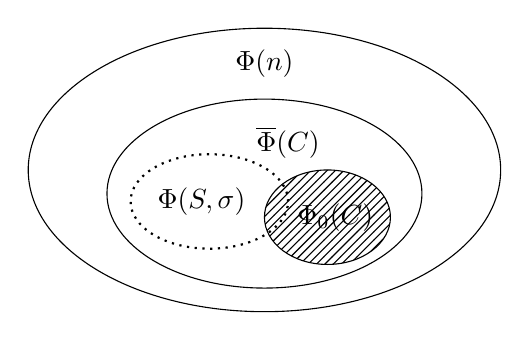
\begin{tikzpicture}[scale=1.0]
        \draw (0, 0) ellipse (3cm and 1.8cm);
        \draw (0, -0.3) ellipse (2cm and 1.2cm);
        \draw[fill opacity=0.4, pattern=north east lines] (0.8, -0.6) ellipse (0.8cm and 0.6cm);
        \draw[dotted, thick] (-0.7, -0.4) ellipse (1.0cm and 0.6cm);

        \node at (0.9, -0.6) { $\Phi_0(C)$ };
        \node at (0.3, 0.35) { $\overline{\Phi}(C)$ };
        \node at (0, 1.35) { $\Phi(n)$ };
        \node at (-0.8, -0.4) { $\Phi(S, \sigma)$ };
    \end{tikzpicture}

    \caption{C-reducibility requires that for some choice of a reducer $(S,\sigma)$, the colorings $\Phi(S, \sigma)$ can be converted to valid ring colorings of $C$ in $\Phi_0(C)$.}
    \label{fig:cred}
\end{figure}

Therefore, C-reducibility can be seen as an extension of D-reducibility with the reducer $(S, \sigma)$ acting as a "filter" of ring colorings. This way we can ignore those ring colorings that are not in $\overline{\Phi}(C)$. As can be seen in Figure \ref{fig:cred}, there are still colorings for the ring that are not in $\overline{\Phi}(C)$. However, we avoid them using the colorings of the reducer $\Phi(S, \sigma)$.

Let us start with the definition of a ring contraction.

\begin{definition}
    A ring contraction $\sigma(v)$ is a map from the vertices of a ring $R$ to the contracted ring $\sigma \circ R$. We require
    
    \begin{itemize}
        \item The contracted ring $\sigma \circ R$ is a valid planar graph.
        \item Neighboring ring vertices $v_i$ and $v_{i+1}$ are not contracted.
    \end{itemize}
\end{definition}

Ring contractions allows the reducer to shrink the number of boundary vertices. This simplifies the coloring problem for the reducer. Without a ring contraction, our reducer would still have the same ring as our configuration $C$, making it equally difficult to work with. Why do we not simply delete vertices from the ring of $C$? The contraction defines a map that allows us to convert boundary colorings of $(S,\sigma)$ to ring colorings of $C$ simply by un-contracting. 

\begin{figure}[!h]
    \centering
    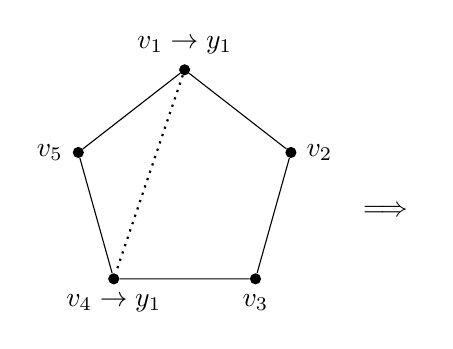
\begin{tikzpicture}[scale=1.5]
        \node[circle, fill, scale=0.015cm, label=above:{$v_1 \rightarrow y_1$}] (l1) at (0, 1) { };
        \node[circle, fill, scale=0.015cm, label=right:{$v_2$}] (l2) at (0.9, 0.30) { };
        \node[circle, fill, scale=0.015cm, label=below:{$v_3$}] (l3) at (0.6, -0.77) {};
        \node[circle, fill, scale=0.015cm, label=below:{$v_4 \rightarrow y_1$}] (l4) at (-0.6, -0.77) {};
        \node[circle, fill, scale=0.015cm, label=left:{$v_5$}] (l5) at (-0.9, 0.30) {};
        \draw (l1) -- (l2) -- (l3) -- (l4) -- (l5) -- (l1);
        \draw[dotted, thick] (l1) -- (l4);
        \node at (1.7, -0.2) { $\implies$ };
    \end{tikzpicture}
    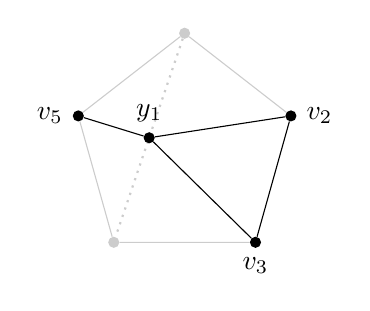
\begin{tikzpicture}[scale=1.5]
        \node[circle, fill, opacity=0.2, scale=0.015cm] (l1) at (0, 1) {};
        \node[circle, fill, opacity=0.2, scale=0.015cm] (l4) at (-0.6, -0.77) {};
        \node[circle, fill, scale=0.015cm, label=above:{$y_1$}] (y1) at (-0.3, 0.115) {};

        \node[circle, fill, scale=0.015cm, label=right:{$v_2$}] (l2) at (0.9, 0.30) { };
        \node[circle, fill, scale=0.015cm, label=below:{$v_3$}] (l3) at (0.6, -0.77) {};
        \node[circle, fill, scale=0.015cm, label=left:{$v_5$}] (l5) at (-0.9, 0.30) {};

        \draw (l5) -- (y1) -- (l2) -- (l3) -- (y1);
        \draw[dotted, thick, opacity=0.2] (l1) -- (l4);
        \draw[opacity=0.2] (l5) -- (l1) -- (l2);
        \draw[opacity=0.2] (l3) -- (l4) -- (l5);
    \end{tikzpicture}
    \caption{A contraction on $R_5$. The two vertices $v_1$ and $v_4$ are mapped to the same vertex $y_1$, and hence get contracted together. }
    \label{fig:contract}
\end{figure}

Figure \ref{fig:contract} shows the contraction process on $R_5$. Intuitively, you should think of a contraction as the merging of pairs of vertices to a single point. However, mathematically, it is easier to work with a mapping function $\sigma$ instead. Suppose we are given a coloring $x(v)$ of a contracted ring $\sigma \circ R$. Then the composition $x \circ \sigma(v)$ is a valid coloring for $R$. This is shown in Figure \ref{fig:contractcolor}

\begin{figure}[!h]
    \centering
    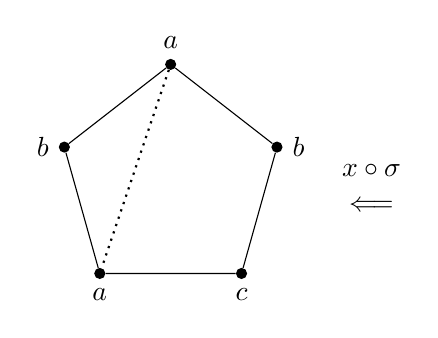
\begin{tikzpicture}[scale=1.5]
        \node[circle, fill, scale=0.015cm, label=above:{$a$}] (l1) at (0, 1) { };
        \node[circle, fill, scale=0.015cm, label=right:{$b$}] (l2) at (0.9, 0.30) { };
        \node[circle, fill, scale=0.015cm, label=below:{$c$}] (l3) at (0.6, -0.77) {};
        \node[circle, fill, scale=0.015cm, label=below:{$a$}] (l4) at (-0.6, -0.77) {};
        \node[circle, fill, scale=0.015cm, label=left:{$b$}] (l5) at (-0.9, 0.30) {};
        \draw (l1) -- (l2) -- (l3) -- (l4) -- (l5) -- (l1);
        \draw[dotted, thick] (l1) -- (l4);
        
        \node at (1.7, 0.1) { $x \circ \sigma$ };
        \node at (1.7, -0.2) { $\Longleftarrow$ };
    \end{tikzpicture}
    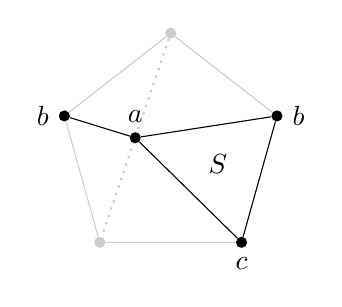
\begin{tikzpicture}[scale=1.5]
        \node[circle, fill, opacity=0.2, scale=0.015cm] (l1) at (0, 1) {};
        \node[circle, fill, opacity=0.2, scale=0.015cm] (l4) at (-0.6, -0.77) {};
        \node[circle, fill, scale=0.015cm, label=above:{$a$}] (y1) at (-0.3, 0.115) {};

        \node[circle, fill, scale=0.015cm, label=right:{$b$}] (l2) at (0.9, 0.30) { };
        \node[circle, fill, scale=0.015cm, label=below:{$c$}] (l3) at (0.6, -0.77) {};
        \node[circle, fill, scale=0.015cm, label=left:{$b$}] (l5) at (-0.9, 0.30) {};

        \draw (l5) -- (y1) -- (l2) -- (l3) -- (y1);
        \draw[dotted, thick, opacity=0.2] (l1) -- (l4);
        \draw[opacity=0.2] (l5) -- (l1) -- (l2);
        \draw[opacity=0.2] (l3) -- (l4) -- (l5);

        \node at (0.4, -0.11) { $S$ };
    \end{tikzpicture}
    \caption{ The coloring $x(v)$ of a contracted ring $\sigma \circ R$ can be converted to a coloring for the original ring $R$ using $x \circ \sigma(v)$. }
    \label{fig:contractcolor}
\end{figure}

By introducing ring contractions, we have already covered the most significant part of a reducer. The last part is the extra graph $S$ that defines the interior of our contracted ring. This extra graph $S$ is similar to the auxiliary graph $A$ that we used during the 1-reducibility proof of $R_5$. The boundary vertices of $S$ must be the same as the contracted ring $\sigma \circ R$. Now we have all the parts needed to define a reducer.

\begin{definition}
    A reducer of a configuration $C$ is a pair $(S, \sigma)$  consisting of a ring contraction $\sigma$ and a graph $S$ on less vertices than $C$ that has a boundary equal to the contracted ring $\sigma \circ R$.
\end{definition}

Of course, every reducer will reduce the size of a configuration $C$. However, for actual reducibility, we can not simply take any reducer. Our reducer $(S, \sigma)$ must satisfy the filtering property mentioned at the beginning of this section. That is, its ring colorings $\Phi(S, \sigma)$ must be contained in $\overline{\Phi}(C)$. Let us define this set.

\begin{definition}
    Let $(S, \sigma)$ be a reducer. The set of un-contracted ring colorings $\Phi(S, \sigma)$ consists of all the colorings $x \circ \sigma$ with $x(v)$ a boundary coloring of $S$.
\end{definition}

Following this definition, C-reducibility is a simple concept.

\begin{definition}
    A configuration $C$ is C-reducible if $\Phi(S,\sigma) \subset \overline{\Phi}(C)$ for some reducer $(S,\sigma)$.
\end{definition}

Now suppose we have a graph $G$ where $C$ is an embedded C-reducible configuration with reducer $(S,\sigma)$. Suppose that two non-neighboring ring vertices of $C$ are connected by an edge in $G$. If we would contract these vertices together, then we would create a loop on the boundary of $S$. We can not color vertices with loops without breaking the rules of a coloring. Therefore, we must take care to avoid such loops.

Since this issue is specific to the way the configuration $C$ is embedded in the graph $G$, we will give a name to the type of embedding that we are after.

\begin{definition}
    A configuration $C$ is $\sigma$-properly embedded in $G$ if two ring vertices of $C$ that are connected by an non-ring edge in $G$ are not contracted by $\sigma(v)$.
\end{definition}

\begin{definition}
    The C-reducible configuration $C$ has a safe reducer  $(S,\sigma)$ if it only occurs $\sigma$-properly embedded in a Birkhoff graph.
\end{definition}

Before we can use C-reducible configurations to reduce counterexamples, we must first prove the existence of a safe reducer. This was a major source of complications in the original proof of the four color theorem by Appel and Haken. This is a strong condition on the structure of a reducer. We will see examples of safe and unsafe reducers in the next section.

\subsection{C-Reducibility of the Birkhoff diamond}
\label{sec:diamond}

Although we have already shown that the Birkhoff diamond is D-reducible, we will use it as a slightly more interesting example of C-reducibility. A reducer for the Birkhoff diamond we have picture below.

\begin{figure}[!h]
    \centering
    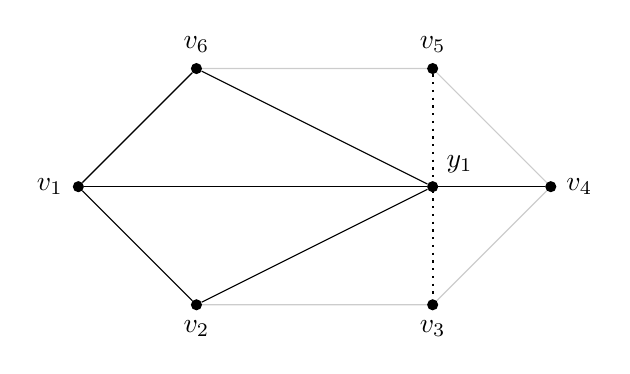
\begin{tikzpicture}[scale=1.5]
        \node[circle, fill, scale=0.015cm, label=left:$v_1$] (l1) at (-2, 0) { };
        \node[circle, fill, scale=0.015cm, label=above:$v_6$] (l2) at (-1, 1) { };
        \node[circle, fill, scale=0.015cm, label=below:$v_2$] (l4) at (-1, -1) {};

        \node[circle, fill, scale=0.015cm,label=right:$v_4$] (r1) at (2, 0) {};
        \node[circle, fill, scale=0.015cm,label=above:$v_5$] (r2) at (1, 1) {};
        \node[circle, fill, scale=0.015cm,label=below:$v_3$] (r4) at (1, -1) {};

        \node[circle, fill, scale=0.015cm,label=above right:$y_1$] (y1) at (1, 0) {};

        \draw[opacity=0.2] (l1) -- (l2) -- (r2) -- (r1) -- (r4) -- (l4) -- (l1);
        \draw[dotted, thick] (r2) -- (r4);
        \draw (l1) -- (l2) -- (y1) -- (l4) -- (l1);
        \draw (l1) -- (y1) -- (r1);
    \end{tikzpicture}
    \caption{A reducer for the Birkhoff diamond (in bold) with a single contraction on $v_4$ and $v_2$, and a single edge added by $S$. }.
    \label{fig:diamondreducer}
\end{figure}

Let us now prove the C-reducibility of the Birkhoff diamond with this reducer. First, we determine the set of colorings that the reducer creates for the original ring $R_6$.

\begin{equation}
    \Phi(S, \sigma) = \left\{ \begin{matrix}
        ababcd, & abcbdc, & abcbcd, \\ abcbac, & abcbad, & \underline{ababac}
    \end{matrix}\right\}
\end{equation}

By looking at Table \
\section{The Birkhoff Diamond}
\label{sec:diamond}

\begin{figure}[!h]
    \centering
    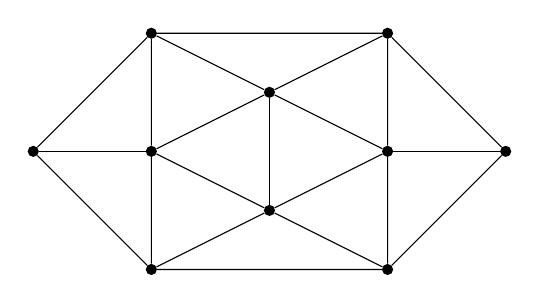
\begin{tikzpicture}[scale=1.5]
        \node[circle, fill, scale=0.015cm] (l1) at (-2, 0) { };
        \node[circle, fill, scale=0.015cm] (l2) at (-1, 1) { };
        \node[circle, fill, scale=0.015cm] (l3) at (-1, 0) {};
        \node[circle, fill, scale=0.015cm] (l4) at (-1, -1) {};

        \node[circle, fill, scale=0.015cm] (r1) at (2, 0) {};
        \node[circle, fill, scale=0.015cm] (r2) at (1, 1) {};
        \node[circle, fill, scale=0.015cm] (r3) at (1, 0) {};
        \node[circle, fill, scale=0.015cm] (r4) at (1, -1) {};

        \node[circle, fill, scale=0.015cm] (c1) at (0, 0.5) {};
        \node[circle, fill, scale=0.015cm] (c2) at (0, -0.5) {};

        \draw (l1) -- (l2) -- (r2) -- (r1) -- (r4) -- (l4) -- (l1);
        \draw (l1) -- (l3);
        \draw (l2) -- (l3) -- (l4);
        \draw (l2) -- (c1) -- (l3) -- (c2) -- (l4);
        \draw (c1) -- (c2);
        \draw (r2) -- (c1) -- (r3) -- (c2) -- (r4);
        \draw (r2) -- (r3) -- (r4);
        \draw (r1) -- (r3);
    \end{tikzpicture}
    \caption{The Birkhoff diamond with ring size 6}.
    \label{fig:diamond}
\end{figure}

\pagebreak
\printbibliography

\end{document}
